 \begin{refsection}
 \chapter{Introduction}

%1)	Introduction
%a.	Function of Voltage-Gated Ion channels
%i.	Action potentials
%ii.	Channelopathies
%iii.	Pharmacology (anesthetics, toxins)
%b.	Structure of Voltage-gated Channels
%i.	Overall topology
%1.	K$^+$ Channel
%2.	Na$^+$ Channel
%ii.	Voltage-gating mechanism
%iii.	Inactivation mechanism
%iv.	Selectivity Filter
%1.	K$^+$ Channel
%2.	Na$^+$ Channel
%c.	History of Ionic Conduction and Selectivity 
%i.	Conduction
%1.	K$^+$ Channel Mechanism
%2.	Na$^+$ Channel Mechanism (previous works)
%ii.	Selectivity
%1.	K$^+$ Channel Mechanism
%2.	Na$^+$ Channel Mechanism (previous works)
%d.	Objective of Study, Outlineff

\section{Enzymes of Early Life}

More than 3 billion years ago, life as we know it began with the formation of membrane-enclosed vesicles \cite{Hille:2001tw,Schopf:2006cx}. An isolated compartment provided an optimal environment for storing genetic materials and performing metabolic activities. However, in order to access necessary substrates and expel waste products, vesicles required a mechanism to transport molecules across the membrane. A unique class of proteins emerged to serve this function, which would later be subcategorized into channels, transporters, and carriers, differing in their cellular role and transport mechanism. Phylogenetic analysis indicates that the last universal common ancestor of life may have possessed more than fifty transport membrane proteins, including the Na$^+$/H$^+$ antiporter and an ATP synthase subunit, which together may have allowed early cells to harness energy in the form of ion gradients \cite{Lane:2012ds,Weiss:2016ie}. Transport proteins like these may have evolved together with primordial membranes to enable more complex cellular functions \cite{Mulkidjanian:2009ko}.

Modern membranes are formed by the self-assembly of lipid molecules. Lipid molecules are amphiphilic, possessing both hydrophobic and hydrophilic groups, and they aggregate into a state where hydrophilic head groups are exposed to water, and greasy hydrophobic tails are buried in the membrane interior \cite{Tanford:1978uu}. In an aqueous environment, ions polarize the water molecules surrounding them, making it energetically unfavorable for these charged complexes to enter the non-polar environment of the membrane \cite{Hauser:1973ul,Paula:1996dn}. Channels can be interpreted as enzymes that catalyze substrate permeation across membranes (Fig. \ref{fig:enzyme}) \cite{Latorre:1983wk,Andersen:1992tf}. In this dissertation, we examine three overarching concepts, common to all channels, which alter the free energy of this catalytic process; permeation, selectivity, and gating.

\begin{figure}[!htb]
\centering
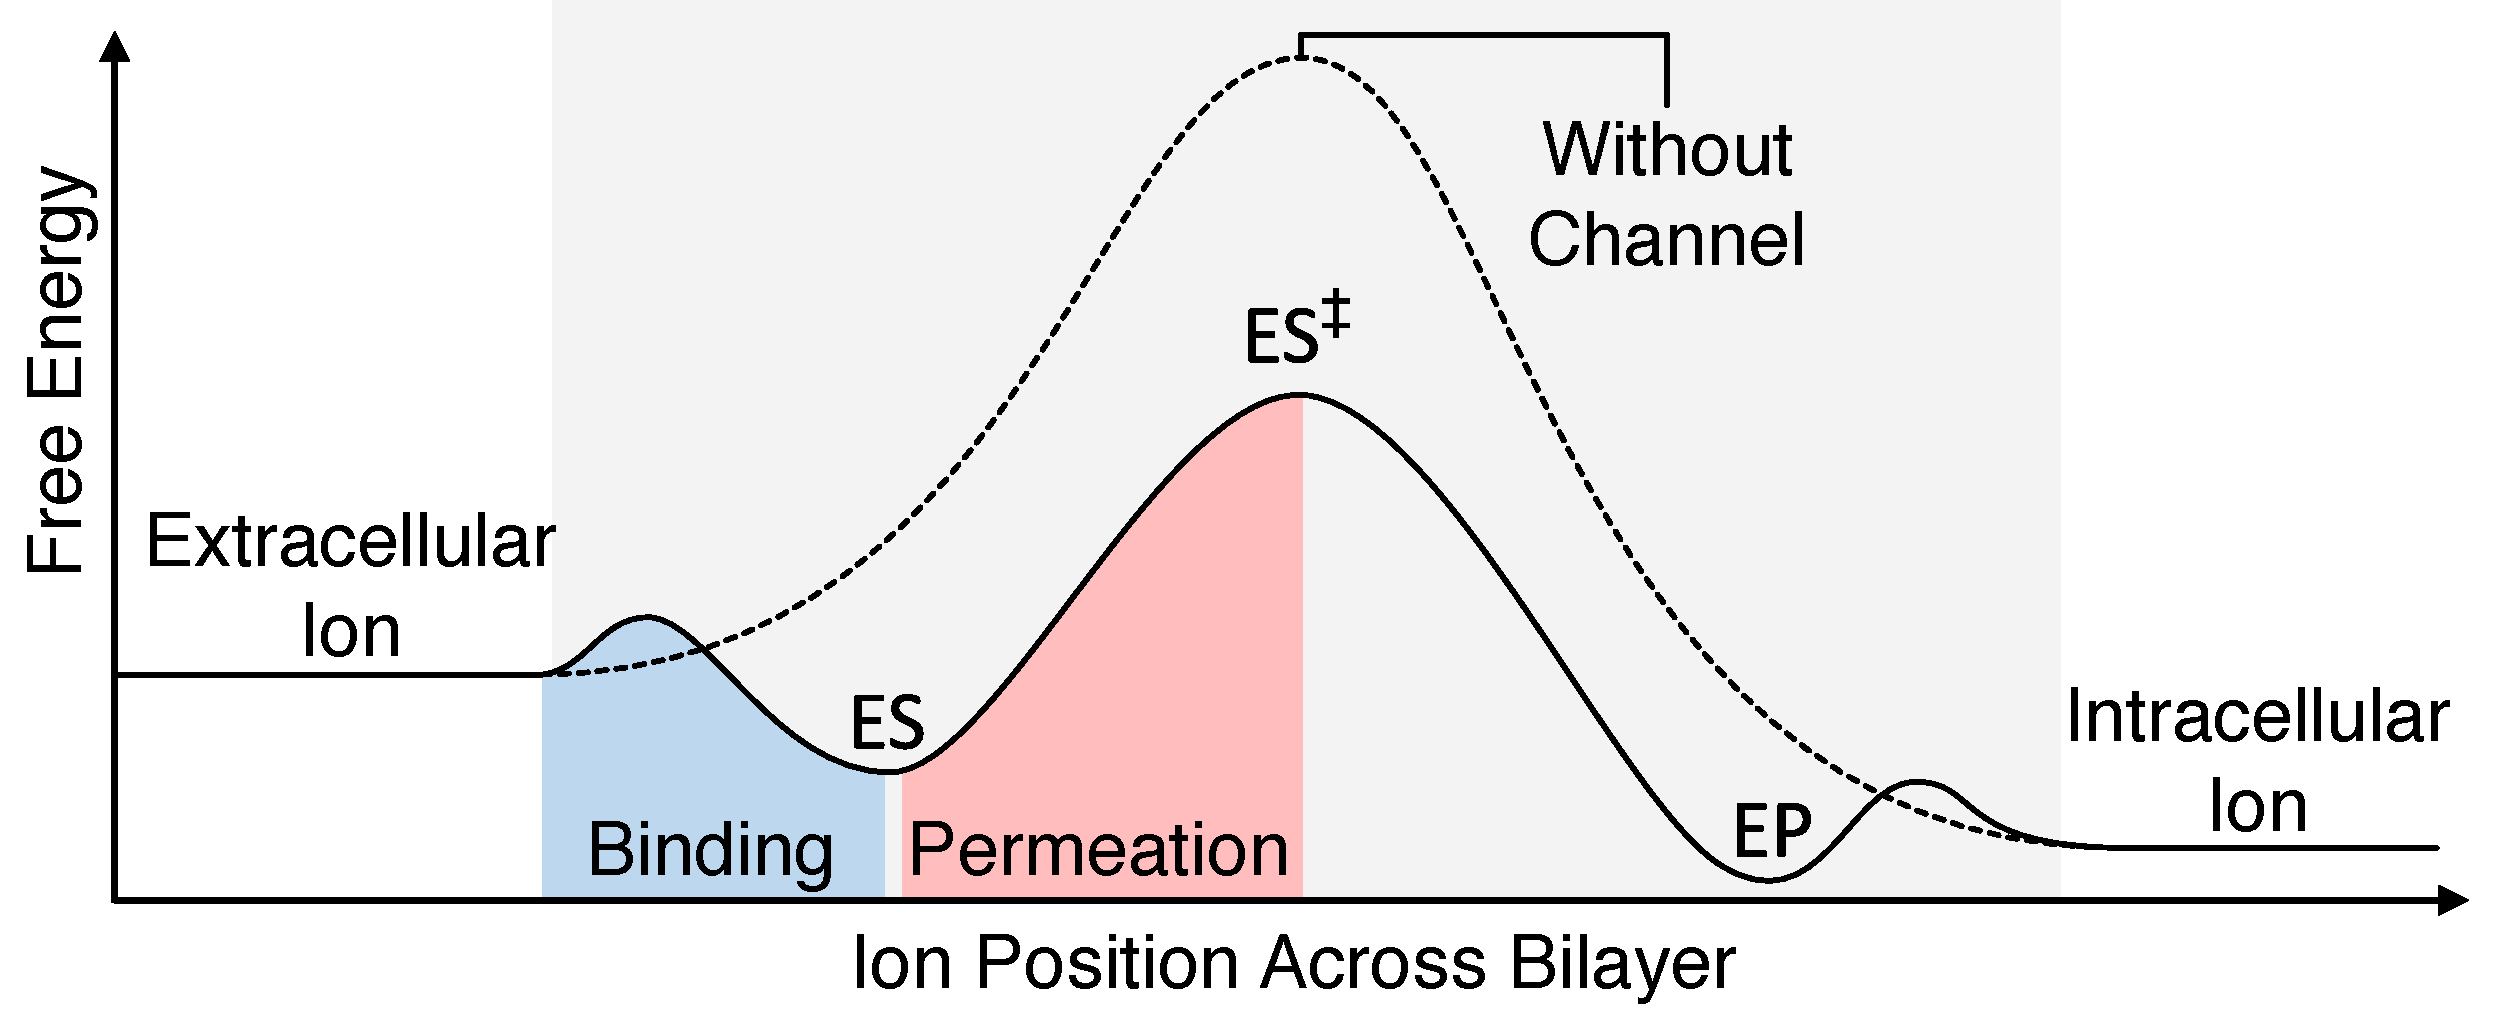
\includegraphics[width=0.6\textwidth]{introduction/enzyme}
\caption[Ion channels are enzymes that catalyze ion conduction]{\textbf{Ion channels are enzymes that catalyze ion conduction}. Schematic diagram depicts the free energy of substrate translocation along a reaction coordinate, with (black solid line) and without (black dashed line) catalysis by an enzyme. Here the reaction coordinate refers to the movement of an ion across a bilayer (grey shaded region) which is catalyzed by an ion channel. Enzyme and substrate ``reactions'' are arbitrarily separated into binding (blue) and permeation (red) events in the terminology of ion conduction.}
\label{fig:enzyme}
\end{figure}

Channels are efficient, permitting ion translocation at a rate of ~10$^6$ ions per second, faster than alternative transport mechanisms like transporters or carriers by several orders of magnitude and faster than turnover rates for well-studied enzymes like trypsin and pepsin \cite{Andersen:1992tf}. Ion channels are capable of operating near the diffusion limit, whereby the translocation rate is restricted by the time it takes for an ion to diffuse through the solvent to the channel opening \cite{Andersen:1983bl}. Once a sufficient number of ions have entered the channel, ion-ion repulsion can assist in the translocation of ions faster than diffusion rate. By nature of their intrinsic charge, ions prefer a polar environment, preferably surrounded by a shell of water molecules. Rapid movement through the confines of a channel can be achieved by maintaining a polar environment for permeating ions. As it can be observed in crystallographic structures of metalloproteins, metals like sodium and potassium preferentially bind to pockets of polar ligands, often in active sites of enzymes. Many of the same design principles hold in ion channels, with the caveat that ions cannot be bound too tightly, or else they may block the channel. More generally, the mechanism of catalysis results from a multitude of energetic contributions that may differ considerably between different families of channels. 

Catalysis by channels depends strongly on the chemical nature of the substrate. Ion channels may range from completely non-selective, allowing any ion of sufficient size to pass, to highly selective, allowing only one ion type to enter. The ions with highest concentration in human cells are Na$^+$, K$^+$, Ca$^{2+}$, and Cl-, which differ in atomic weight, formal charge, and effective radius \cite{Hille:2001tw}. The effective ionic radii are 1.02, 1.38, and 1.00 \AA\ for Na$^+$, K$^+$, and Ca$^{2+}$, respectively \cite{Shannon:1976dq}. Despite having different charges, Na$^+$ and Ca$^{2+}$ have a similar radius, suggesting that Na$^+$ and Ca$^{2+}$ selective channels may share some common features. By contrast, although Ca$^{2+}$ and K$^+$ have similar atomic weights, K$^+$ has a larger spread of electron density due to its monovalent charge which results in a qualitatively larger radius than both Ca$^{2+}$ and Na$^+$. Characterization of ions by effective radii enables the estimation of ion binding sites, but it does not provide information about how strongly they bind. The amount of free energy required to transfer a mole of ions from vacuum to a volume of water is called the hydration free energy. The experimental Gibbs free energy of hydration for Na$^+$, K$^+$, and Ca$^{2+}$ are -365, -295, -1505 kJ mol $^{-1}$, respectively \cite{Marcus:1991kp}. Na$^+$ has a lower hydration free energy than K$^+$, suggesting that it forms moderately stronger interactions with water molecules. The divalent charge of Ca$^{2+}$ strongly polarizes surrounding water molecules resulting in strong interactions. Both the ionic radius and hydration free energy are two of many factors that channels may evolve to accommodate in order to achieve selectivity. The mechanism by which channels are selective is poorly understood.

The passage of ions through channels commonly occurs through a pore formed by the assembly of multiple protein tertiary or quaternary structure elements. Some pores remain constitutively open, while others can open and close in response to a stimulus, like mechanical stretch, ligand binding, pH, ionic concentration, temperature, and voltage \cite{Zheng:2015vj}. These gating mechanisms provide a means for the cell to regulate the flow of substrates in and out of the cell and to ultimately achieve cellular homeostasis. For example, multiple transport proteins are involved in maintaining the optimal concentrations of water, ions and other molecules required for cellular processes to occur. In mammalian skeletal muscle, the extracellular ion concentrations of Na$^+$ and K$^+$ are 145 mM and 4 mM, while intracellular ion concentrations are 12 mM and 155 mM, respectively \cite{Hille:2001tw}. Two of several membrane proteins functioning to hold this concentration imbalance are voltage-gated Na$^+$ and K$^+$ channels (which by convention are denoted as Na\textsubscript{V} and Kv channels). These channels open and close in response to a difference in charge across the membrane. Gating can occur at any position within a channel pore, and may involve conformational change in one region or concerted motions of multiple subunits. All types of gating may halt the movement of substrates across the bilayer, and genetic mutations that alter gating are frequent causes of disease \cite{Ashcroft:2000ts}.

Permeation, selectivity, and gating are fundamental concepts that underlie the functional catalysis of substrates across biological membranes. A deeper understanding of these concepts will assist in improved treatment of patients suffering from defective ion channels and provides a foundation for rational design of channel directed therapeutics.
%One more big picture sentence?

\section{Physiological Role of Ion Channels and Disease}

Over billions of years, channels have evolved to match the growing complexity of cells, transporting diverse substrates under unique regulation mechanisms. Large-scale genome sequencing has provided a means to predict channel genes, driving researchers to clone, express, and functionally characterize many prokaryotic and eukaryotic channels. In human cells, the superfamily of voltage-gated ion channels has been identified and can be interpreted using evolutionary analysis (Fig. \ref{fig:channelome_ap} A) \cite{Yu:2004ep}. This family includes voltage-gated sodium, potassium, and calcium channels, as well as cyclic nucleotide-modulated channels, two-pore channels, and transient receptor potential channels. These channels are expressed in human cells throughout the body and serve diverse functions \cite{Zheng:2015vj,Hille:2001tw}. One of the most ancient of these functions originated shortly after multicellular life evolved, approximately 600 million years ago \cite{Chen:2014du}, enabling cell-to-cell communication and ultimately permitting the evolution of the nervous system.

\begin{figure}[hp]
\centering
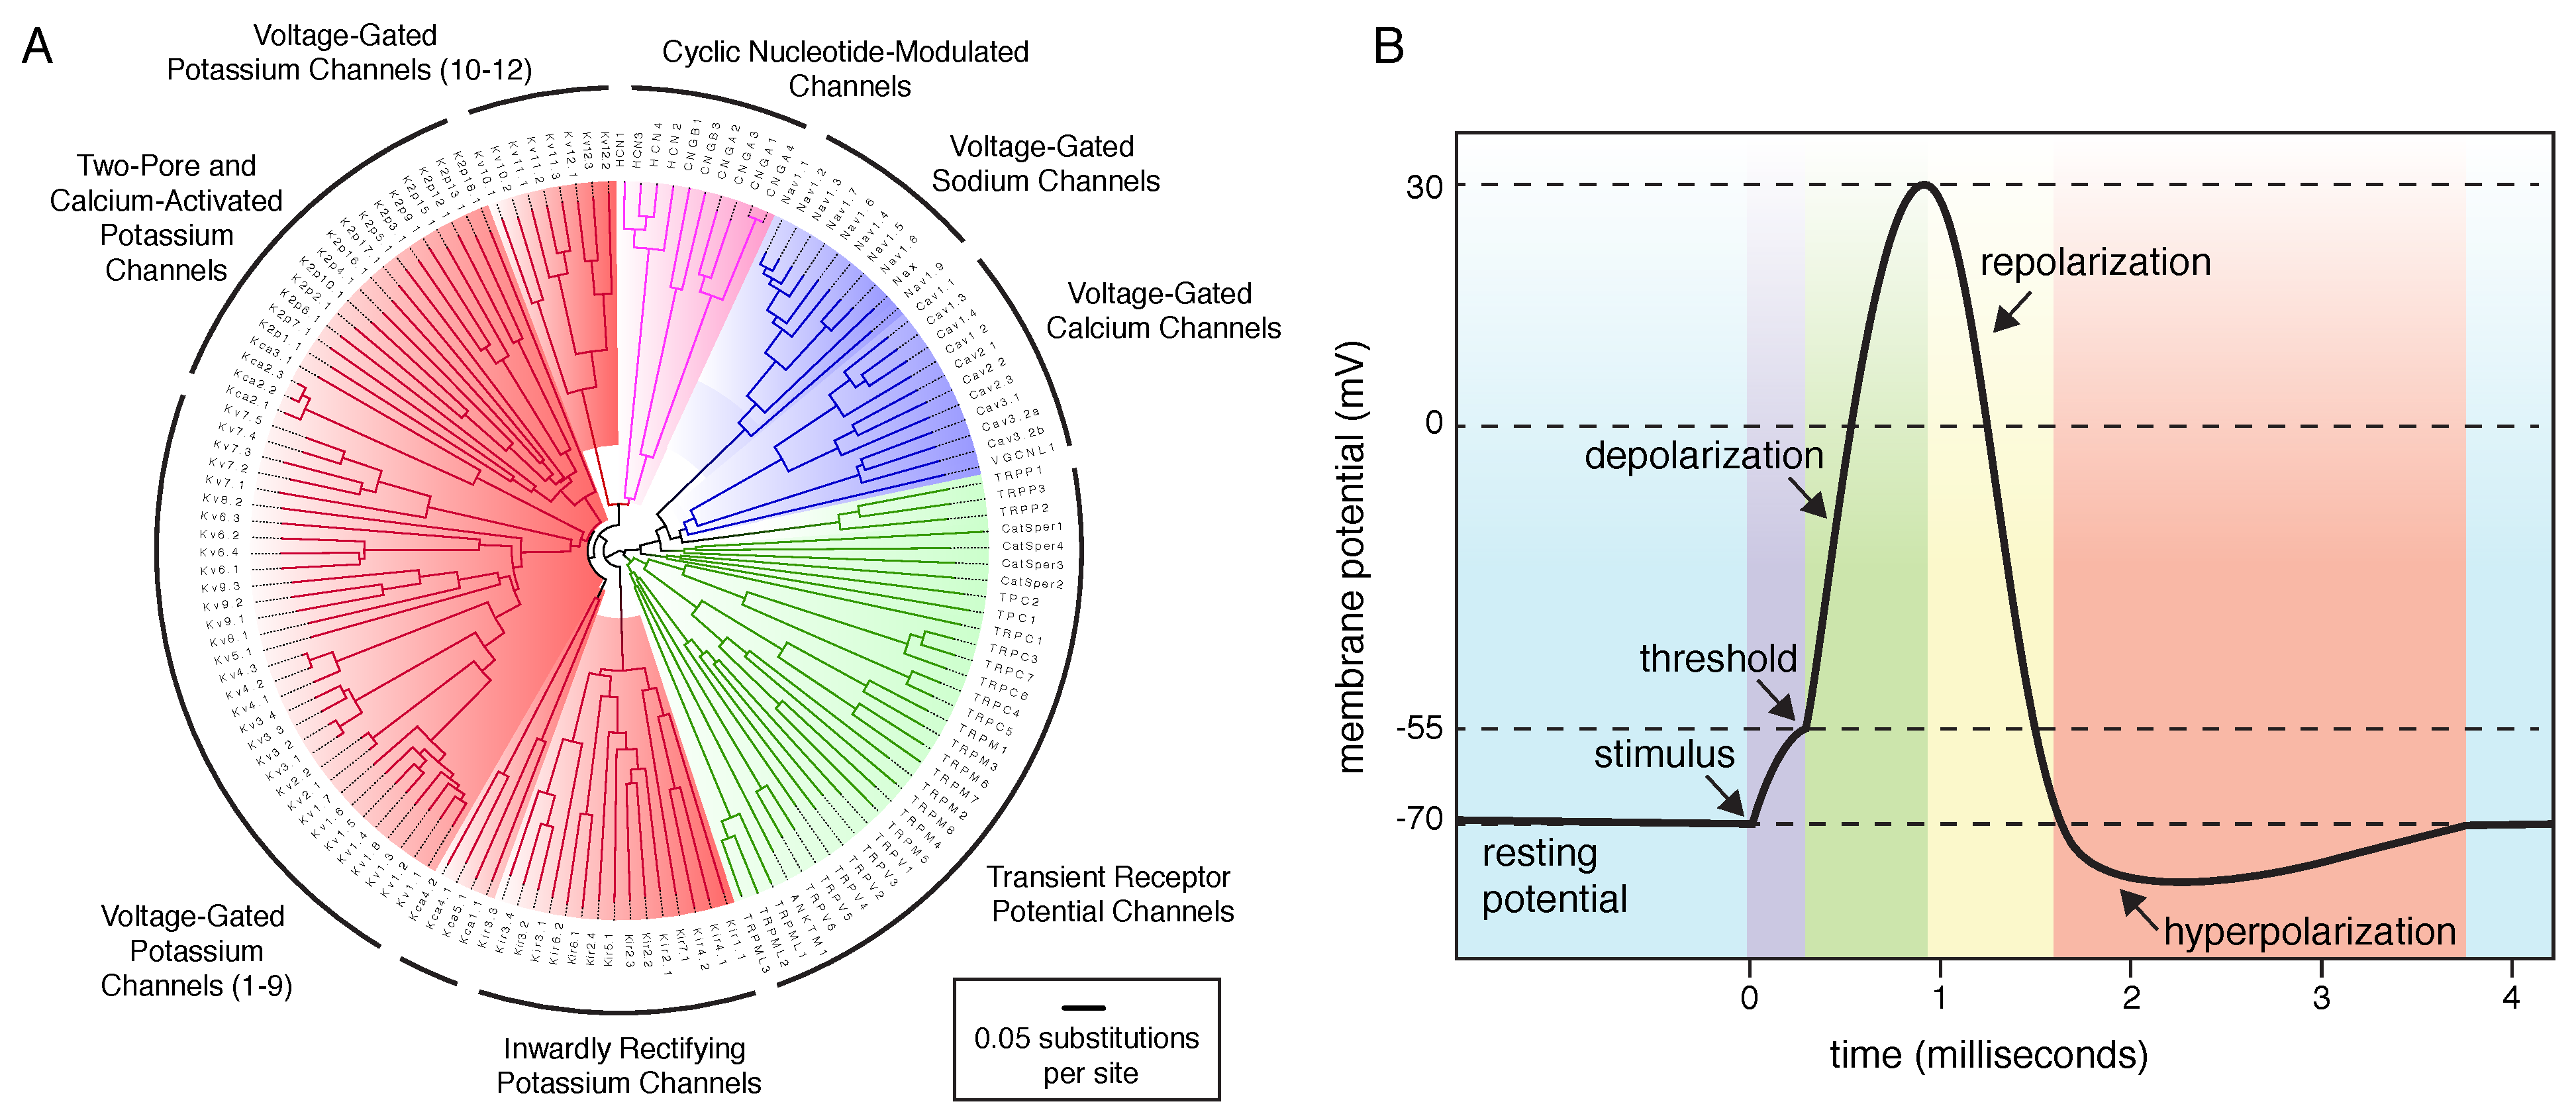
\includegraphics[width=0.9\textwidth]{introduction/channelome}
\caption[Phylogeny of voltage-gated ion channels and action potential schematic]{\textbf{Phylogeny of voltage-gated ion channels and action potential schematic}. (\textbf{A}) Phylogenetic tree of the voltage-gated ion channel superfamily present in the human genome. A set of amino acid sequences from the minimal pore regions of 142 voltage-gated ion channels were collected and sequence aligned \cite{Yu:2004ep}. A phylogenetic tree was constructed, without bootstrapping, using the BIONJ algorithm implemented in SplitsTree \cite{Gascuel:1997ua}. The tree was polarized and coloured using the software FigTree. Voltage-gated ion channel clades are labelled: potassium channels (red), cyclic nucleotide-modulated channels (pink),  sodium and calcium channels (blue), and transient receptor potential channels (green). (\textbf{B}) Schematic representation of an action potential. The course of the action potential is split into five phases; the resting phase (blue), the stimulus phase (purple), the depolarization phase (green), the repolarization phase (yellow), the refractory period (red), and back to the resting phase (blue). Sodium channels and potassium channels are predominately open during the depolarization and repolarization phase, respectively.}
\label{fig:channelome_ap}
\end{figure}

Voltage-gated sodium channels (Na\textsubscript{V} channels) were first characterized by Hodgkin and Huxley in a series of landmark papers published in 1952 \cite{Hodgkin:1952td,Hodgkin:1952vd,Hodgkin:1952um,Hodgkin:1952uf,Hodgkin:1952tr}.  Using the voltage-clamp technique on the membrane of the squid giant axon, Hodgkin and Huxley were able to describe complex phenomena in sodium channels such as voltage-dependent activation, fast inactivation, and Na$^+$ selectivity over other ions. In excitable cells, like neurons, muscle cells, and endocrine cells, Nav and Kv channels result in fast and transient reversals of membrane potential called ``nerve impulses'' or ``action potentials'' in the order of 2-5 milliseconds \cite{Bezanilla:2008ht,Hille:2001tw,Catterall:2012cd}. In neurons, the action potential has a characteristic membrane voltage profile when examined as a function of time, and proceeds sequentially through the following steps (Fig. \ref{fig:channelome_ap} B):
\begin{itemize}
\item \textbf{Stimulus}. An excitatory postsynaptic channel or an action potential from a nearby region causes a localized depolarization of the membrane from its resting state (-70 mV). Many failed activations may occur before the membrane voltage reaches a critical threshold of -44 mV.
\item \textbf{Depolarization}. Once the voltage threshold is reached, Na\textsubscript{V} channel opening probability increases. In the presence of open channels, a difference in ion concentrations and asymmetry of charge across the membrane drives ions through the pores. This driving force is called the electrochemical gradient. While Na$^+$ flows through open Na\textsubscript{V} channels, the membrane becomes even more depolarized, and triggers a positive feedback loop that causes nearby Na\textsubscript{V} channels to open. The highest Na$^+$ currents occur near a membrane potential of 0 mV.
\item \textbf{Repolarization}. At such depolarizing voltages, Kv channels opening probability increases. Open Kv channels permit K$^+$ to flow down its electrochemical gradient to outside of the cell. Outflow of K$^+$ repolarizes the membrane causing Na$^+$ channels to inactivate and subsequently close.
\item \textbf{Undershoot}. As the membrane potential approaches its resting state, some K$^+$ channels close, but prolonged opening causes polarization beyond the resting membrane potential, referred to as hyperpolarization.
\item \textbf{Refractory Period}. After a prolonged interval, the resting membrane potential is gradually restored at the site of interest (-70 mV). During this time, inactivated Na\textsubscript{V} channels cannot be made to activate at any membrane potential. The self-propagating nature of this mechanism drives the action potential to traverse the length of the neuron, and the refractory period helps ensure that the action potential will not move backwards.  
\end{itemize}

Action potentials play a vital role in human physiology. In neurons, this process permits long-distance signalling in the nervous system. In cardiac and skeletal muscle cells, action potentials play a critical role in muscle contraction. In pancreatic $\beta$ cells, the action potential stimulates the release of insulin. At the molecular level, these critical physiological processes rely on selective transport of ions, and thus it is not surprising that impairment of sodium flux through Na\textsubscript{V} channels can result in devastating human diseases. Mutations in the genes encoding for human Na$^+$ channels can result in diseases broadly classified as epileptic/non-epileptic, muscle, or pain disorders \cite{Ashcroft:2000ts}. Epileptic and non-epileptic disorders range from generalized epilepsy with febrile seizures (GEFS+) and Dravet syndrome to familial hemiplegic migraine and autism. Muscle disorders include hyper- and hypo- kalemic periodic paralysis, long QT syndrome (abnormal repolarization of the heart), along with paramyotonia congenita (prolonged muscle contraction). Pain disorders include congenital insensitivity to pain, and paraoxysmal extreme pain disorder. Na\textsubscript{V} channels have also been identified as serving non-canonical roles in non-excitable cells like astrocytes, T cells, macrophages, and cancer cells \cite{Black:2013gp}. In bacteria, prokaryotic Na\textsubscript{V} channels function to maintain sodium ion concentration and pH homeostatis \cite{Ito:2004da}, but may serve additional functions that are not understood.

The central physiological role of Na\textsubscript{V} channels position them as important drug targets. Human sodium channels are blocked by drugs used clinically as local anesthetics, antiarrythmics, and antiepileptics \cite{Catterall:2014eq}. In several drug binding sites, eukaryotic and prokaryotic Na\textsubscript{V} channels have very similar pharmacological characteristics. Electrophysiological studies reveal that the local anesthetics lidocaine \cite{Lee:2012bs}, isoflurane \cite{Ouyang:2007he}, and sevoflurane \cite{Barber:2014us}, can inhibit the bacterial sodium channel NaChBac in a similar manner to eukaryotic Na\textsubscript{V} channels. Functional electrophysiological studies reveal that the prokaryotic channel Na\textsubscript{V}Ms binds and is inhibited by small hydrophobic sodium channel blockers in a similar manner to human Nav1.1 \cite{Bagneris:2014ks}. Tested channel blockers include the clinically relevant lamotrigine and lidocaine, commonly used anticonvulsant and anesthetic drugs, respectively. Similarly, functional and structural characterization reveals that the prokaryotic calcium channel Ca\textsubscript{V}Ab is blocked by human Cav1.2 channel inhibitors \cite{Tang:2016el}. Given the pharmacological similarity of eukaryotic and prokaryotic Na\textsubscript{V} channels, recent structural determination efforts focused on prokaryotic channels provide a useful basis for understanding human Na\textsubscript{V} channel related diseases and designing therapeutics.

\section{Voltage-gated Ion Channel Structure and Function}

In 1971, before any ion channel sequence or structure was determined, Hille was able to construct a structural model of the narrowest constriction in Na\textsubscript{V} channels, the selectivity filter or SF, by measuring the permeability of a range of organic cations \cite{Hille:1972wz,Hille:1971vq}. Hille predicted a rectangular selectivity filter of dimensions 3 $\times$ 5 \AA\ that was lined with oxygen atoms, and predicted that permeating Na$^+$ could be partially hydrated and make direct contacts with up to three oxygen ligands of the selectivity filter.  In a follow-up study, Hille measured the permeability of a range of metal cations through sodium channels and found a characteristic ordering of selectivity (Na$^+$ $\approx$ Li$^+$ $>$ Tl$^+$ $>$ K$^+$ $>$ Ca$^{2+}$) \cite{Hille:1972wz,Eisenman:1962dy}. Based on the ``field strength'' theory of Eisenman \cite{Noda:1987gc,Eisenman:1983tc}, strong negatively charged ligands, like carboxyl oxygen atoms, could create ``high field'' binding sites for small cations preferentially, and Hille found that his results were consistent with this model. This work, along with many studies like it, laid the foundation for the structural investigation of ion permeation and selectivity in ion channels.

Cloning and expression of mammalian Na\textsubscript{V} channel led to the identification of a toxin binding site within the pore \cite{Noda:1986jn,Noda:1986ct,Terlau:1991ud,Noda:1989bj}. Through both mutagenesis and selectivity measurements for organic and inorganic cations, this site formed by a ring of residues with sequence ``DEKA'' was determined to be the selectivity filter \cite{Terlau:1991ud,Schlief:1996tb,Sun:1997uj}. Alignment of several calcium channel sequences revealed an ``EEEE'' ring at the same position within the putative calcium channel SF, and thus motivated site-directed mutagenesis to modify the eukaryotic sodium channel SF at this location \cite{Heinemann:1992ep}. The mutation of ``DEKA'' to ``DEEA'' or ``DEEE'' was sufficient to confer selectivity properties characteristic of a calcium channel, suggesting that this region alone is sufficient to impart selectivity. A mutation of the glutamic acid in ``DEKA'' to remove this high-field strength channel ligand was also found to decrease Na$^+$ selectivity over K$^+$ \cite{Favre:1996dg} in agreement with the Eisenman model. Conversely, subsequent experiments suggest the ``EEEE'' ring alone is sufficient to confer calcium selectivity in Cav channels \cite{Yang:1993ux,Ellinor:1995ky,Cibulsky:2000ix}, suggesting high structural homology between Nav and Cav channels. However, the distinction between Nav and Cav channels is often blurred across the kingdoms of life.

Phylogenetic analysis suggests that Na\textsubscript{V} channels evolved from Cav channels \cite{Hille:1989vz,Hille:2001tw,Yu:2004ep,Liebeskind:2011dn,GurBarzilai:2012kh} (Fig. \ref{fig:channelome_ap} A), but functional characterization of channels reveals greater complexity. The characteristic ``DEKA'' SF sequence is conserved in all vertebrate and many invertebrate Na\textsubscript{V} channels \cite{Widmark:2010in} and the ``EEEE'' and ``EEDD'' SF sequence are conserved in Cav1/Cav2 and Cav3 channels, respectively, in all known animal species back to the single-cell organisms which they originated \cite{Stephens:2015iv}. An evolutionary relationship between Cav and Na\textsubscript{V} channels is supported by putative "evolutionary intermediates" containing a ``DEEA'' SF sequence in several invertebrates. One of these channels, the German cockroach Na$^+$ channel 1 (BSC1), has high sequence similarity to Na\textsubscript{V} channels and is permeable to both Na$^+$ and Ca$^{2+}$ but could be functionally classified as a Cav channel \cite{Zhou:2004tc}. On the contrary, the \emph{Apis mellifera} Na\textsubscript{V} channel has the same ``DEEA'' motif, but is selective for Ca$^{2+}$ and impermeable to Na$^+$ \cite{GosselinBadaroudine:2016gw}, suggesting that regions outside of the SF influence selectivity. Indeed, modifications to residues in close vicinity to the SF were required to achieve Na$^+$ selectivity in a related invertebrate channel classified as a Na\textsubscript{V} channel \cite{GurBarzilai:2012kh}. Additionally, the evolutionary relationship between prokaryotic and eukaryotic Nav and Cav channels is unclear, however some studies suggest that eukaryotic sodium and calcium channels share prokaryotic sodium channels as a common ancestor \cite{Ren:2001uo,Yu:2004ep,Koishi:2004hy,Catterall:2015dh,Charalambous:2011dc}. The bacterial sodium channel NaChBac and several prokaryotic relatives were found to possess the same ``EEEE'' motif as observed in SF of Cav channels \cite{Ren:2001uo}. Bacterial sodium channels form homo-tetrameric assemblies of transmembrane helices S1-S6, whereas the mammalian Nav and Cav channels consist of a hetero-tetrameric assembly of a single chain containing 24 transmembrane helices \cite{Guy:1986bl,Ren:2001uo,Koishi:2004hy}. Mutagenesis studies reveal that the SF of prokaryotic Na\textsubscript{V} channels can be modified to impart Ca$^{2+}$ selectivity by introducing multiple ``DDDD'' rings within the SF \cite{Tang:2014cn,Shaya:2011ih,Yue:2002ee}. As such, bacterial voltage-gated sodium channels offer an promising model for gaining an understanding of the principles of Na$^+$ permeation and selectivity in the larger sodium and calcium channel superfamily.

% Thinking about full-on director's commentary in the comments of my thesis. (This negative result took 5000 CPU years, Reviewers ate us alive on this,) 

\subsection{Voltage-gated Ion Channel Structures}

% Explain features of Na\textsubscript{V}Ab, 
Sixty years after the seminal work of Hodgkin and Huxley, the first three-dimensional structure of a bacterial voltage-gated sodium channel, Na\textsubscript{V}Ab, was solved by x-ray crystallography \cite{Payandeh:2012ib,Catterall:2012fh}. The structure of Na\textsubscript{V}Ab consists of four identical subunits, each contributing one pore domain monomer and one voltage sensing domain (Fig. \ref{fig:nav_sf} A, extracellular view). All of the pore domain monomers, each comprised of transmembrane helices S5 and S6, form the ion conduction pore along the principal axis of the channel. Permeating sodium ions flow down their electrochemical gradient from the extracellular to intracellular side of the membrane, passing through several regions of the pore (Fig. \ref{fig:nav_sf} C, side view). Ions are first recruited to the pore entrance by negatively charged residues in the extracellular vestibule (EC). Past this point, ions enter through the narrowest constriction of the pore, named the selectivity filter (SF). The SF and surrounding features of the EC, comprised by pore helix P1 and P2, contribute the primary structural determinants for Na$^+$ selectivity. Beyond the SF, ions enter a water-filled expansion within the channel, named the central cavity (CC). Below the CC at the intracellular end of the pore, is another narrow constriction called the activation/intracellular gate (AG/IC). This constriction is formed by close packing of S6 helices when the pore domain is in a closed state, and dilates to some extent in the open state. Each subunit of the central pore domain is connected to a voltage-sensing domain, comprised of transmembrane helices S1-S4, by a structured S4-S5 linker. In Na\textsubscript{V}Ab and all known bacterial Nav structures, the voltage-sensing domains are ``domain-swapped'', making contact with the pore domain of the neighbouring pore domain monomer. Upon membrane depolarization, S4 transmembrane helices undergo conformational change which is translated to the intracellular gate of the pore domain through rearrangement of S6 helix packing \cite{Vargas:2012ek,Long:2005hl,Jensen:2012ee,Catterall:2015dh}. 

% Quick paragraph on K$^+$ channel stuctures
Nav and Kv channels share a similar domain architecture with a central pore domain and four voltage sensing domains (Fig. \ref{fig:nav_sf} A-D). The first crystallographic structure of a K$^+$ channel, KcsA, was solved more than a decade before the sodium channel structure \cite{Doyle:1998wq}. Building on the work of this landmark paper, structures from multiple families of K$^+$ channels represented in the phylogeny of human voltage-gated ion channels have now been solved (Fig. \ref{fig:channelome_ap} A) \cite{Tian:2013er,Kuang:2015jn}. This includes structures of several voltage-gated potassium channels [KvAP \cite{Jiang:2003vh}, Kv1.2 \cite{Long:2005do}, the Kv1.2/Kv2.1 chimera (Fig. \ref{fig:nav_sf} B,D) \cite{Long:2007cv}, and KvLm \cite{Santos:2012gg}]. Kv channels of known structure have similar overall architecture to bacterial Na\textsubscript{V} channels but differ considerably in the SF (Fig. \ref{fig:nav_sf} B).

\begin{figure}[hp]
\centering
\includegraphics[width=0.9\textwidth]{introduction/navsf}
\caption[Molecular rendering of voltage-gated ion channels and selectivity filter structure of Na$^+$ and K$^+$ selective channels]{\textbf{Molecular rendering of voltage-gated ion channels and selectivity filter structure of Na$^+$ and K$^+$ selective channels}. Molecular snapshots of the tetrameric assembly of (\textbf{A}) sodium channel Na\textsubscript{V}Ab \cite{Payandeh:2012ib} and (B) a potassium channel chimera, Kv1.2/Kv2.1 \cite{Long:2007cv} from the extracellular view. (\textbf{C-D}) Snapshots of Na\textsubscript{V}Ab and Kv1.2/Kv2.1 channels embedded in a lipid bilayer after coarse-grained molecular dynamics \cite{Stansfeld:2015tb}. Only two of four subunits are depicted from a side-orientation to assist in visualizing the protein interior. Lipid molecules are shown in white and water molecules in red and white. Cylinders depict the helices forming the voltage-sensing domain (helices S1-S4, orange), the S4-S5 linker (blue), pore- domain helix S5 (red), the pore helix (purple), and pore-domain helix S6 (yellow). Na\textsubscript{V}Ab contains an additional helix near the selectivity filter (green). A dashed box indicates the position of the selectivity filter. Molecular renderings of two opposite subunits of the selectivity filter in (\textbf{E}) Na\textsubscript{V}Ab \cite{Payandeh:2012ib} and (\textbf{F}) KcsA \cite{Zhou:2001vo}. Residue numbers are shown for pore-lining channel ligands. Within the SF, each label indicates an observed or putative ion binding site.}
\label{fig:nav_sf}
\end{figure}

\begin{figure}[hp]
\centering
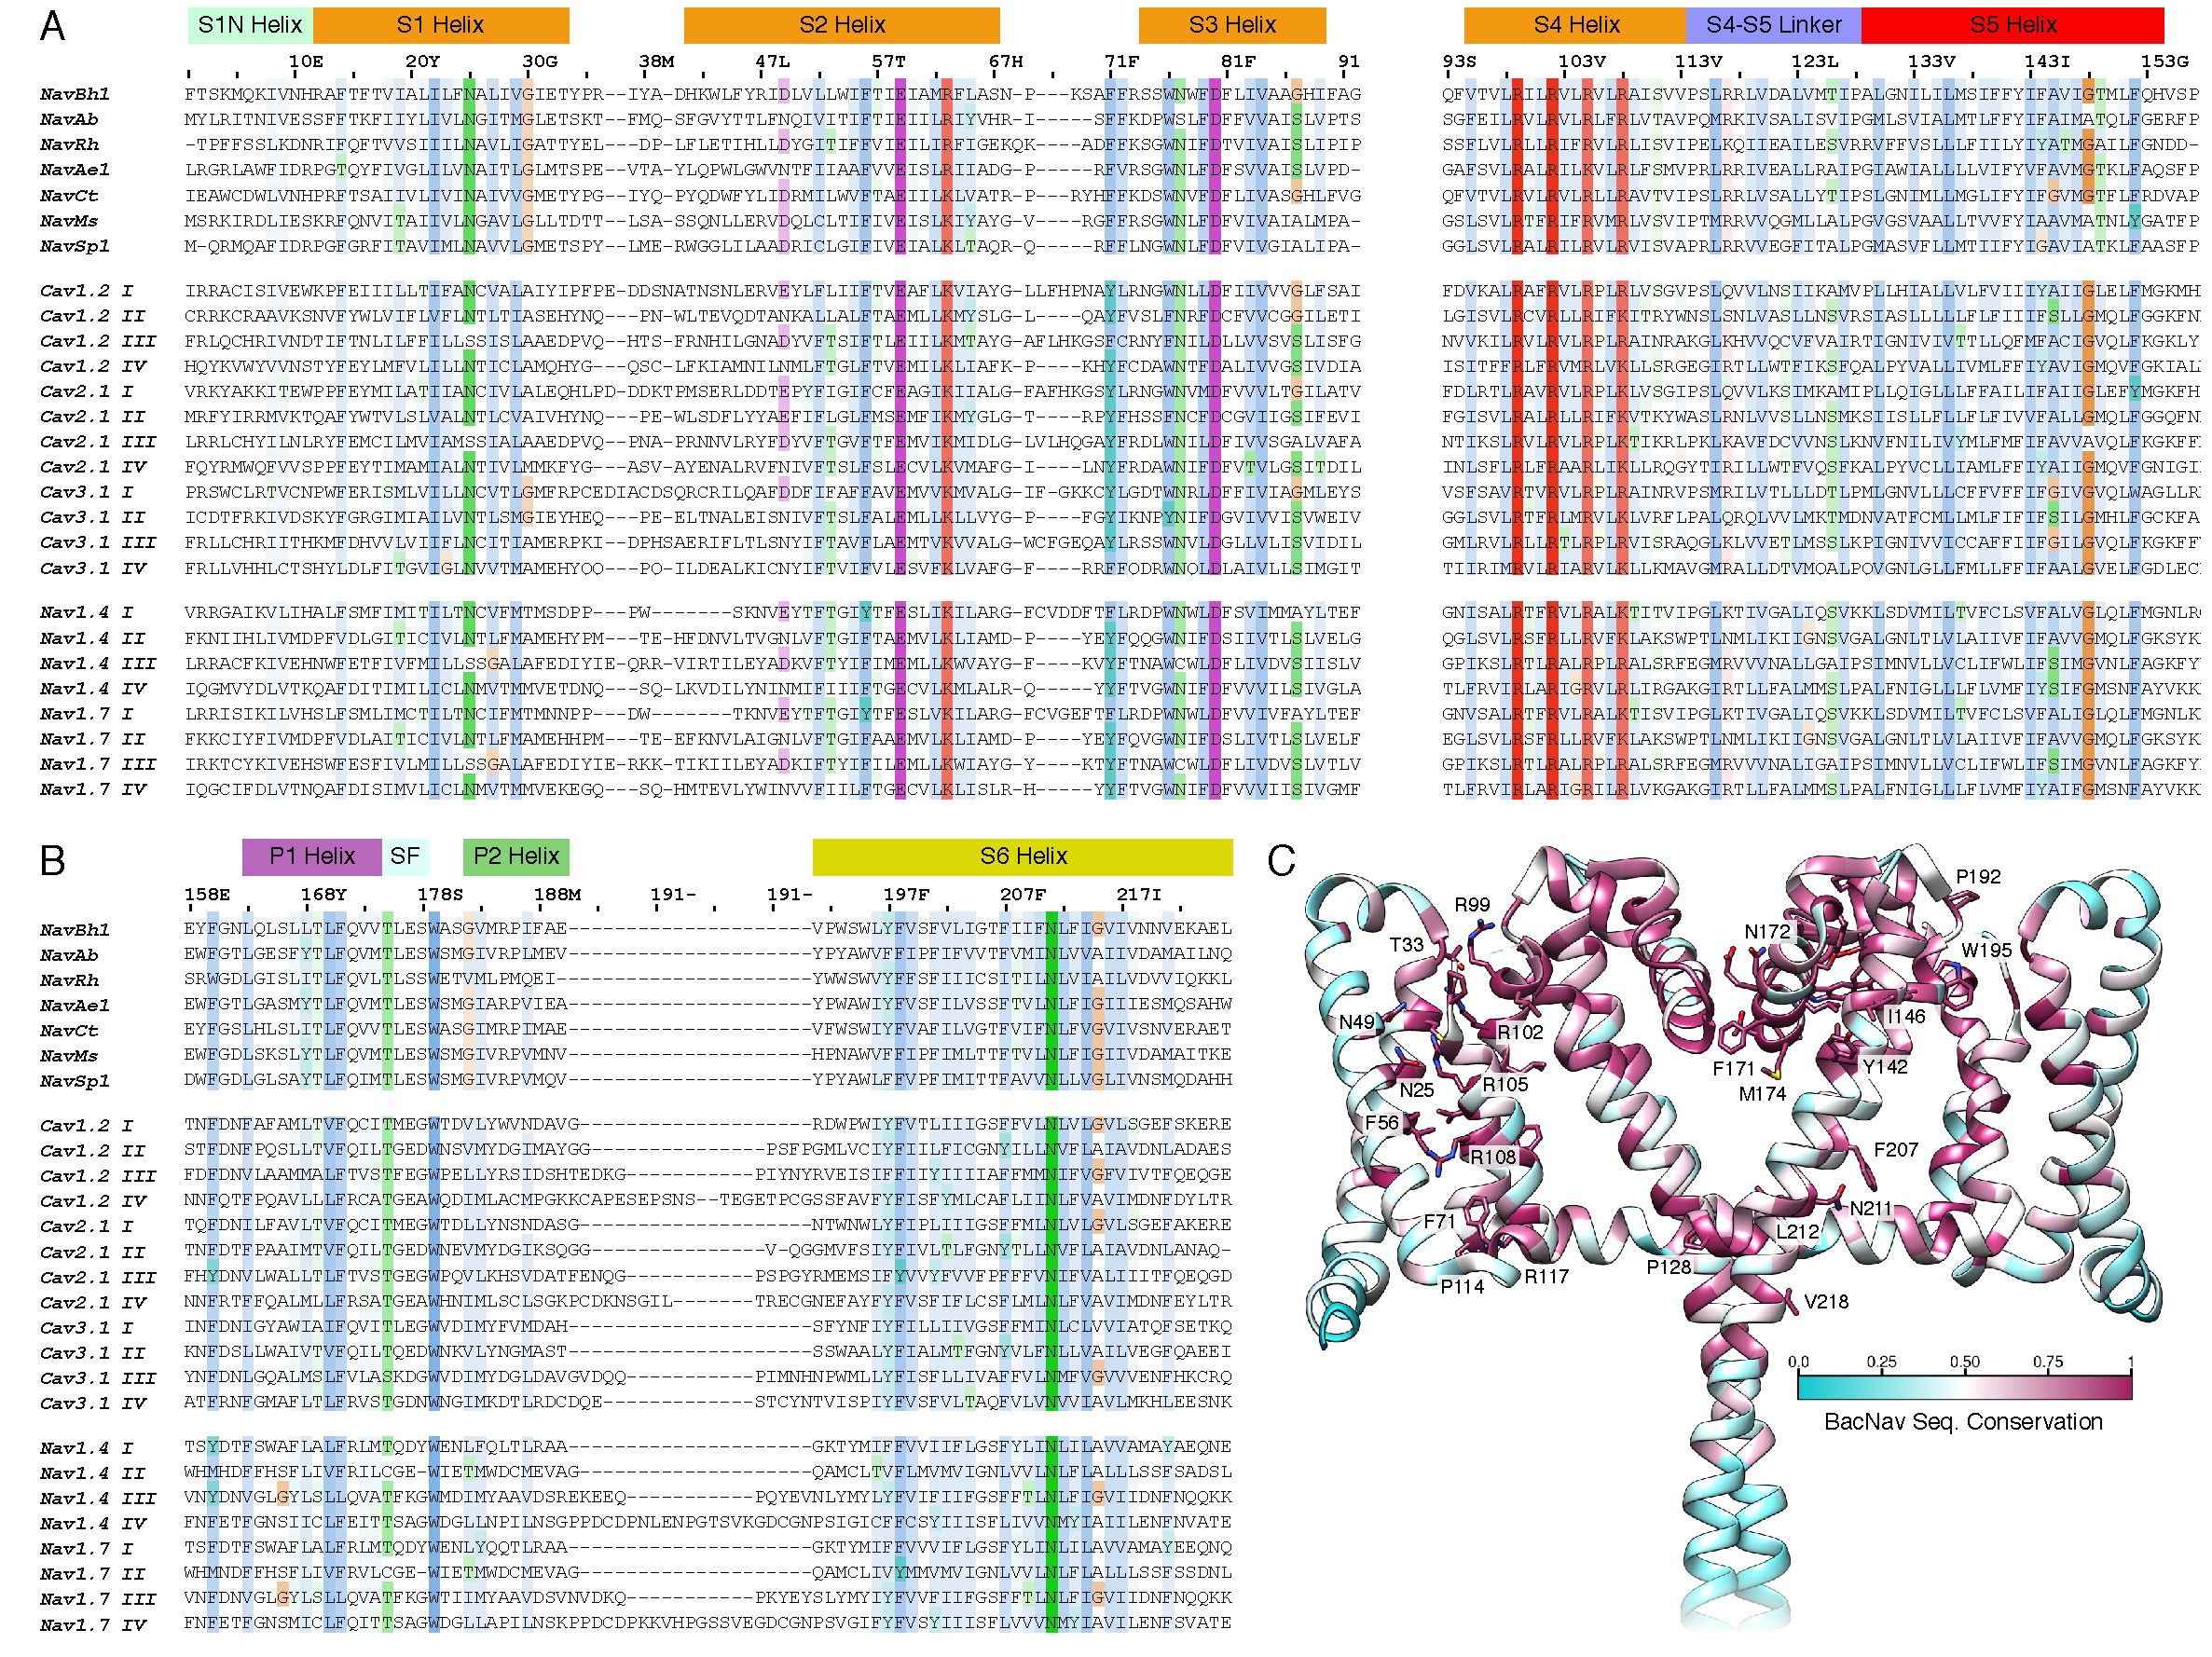
\includegraphics[width=1.0\textwidth]{introduction/sequence}
\caption[Voltage-gated sodium and calcium channel sequence alignment and conservation]{\textbf{Voltage-gated sodium and calcium channel sequence alignment and conservation}. Sequence alignment of structurally and functionally characterized homo-tetrameric prokaryotic sodium channels along with multiple heterotetrameric human Nav and Cav channels. (\textbf{A}) Sequence alignment is shown using Na\textsubscript{V}Ab as a reference for both the numbering and secondary structure assignments of the (\textbf{A}) S1-S5 and (\textbf{B}) P1-S6 helices. (\textbf{C}) A molecular rendering of two diagonal subunits from the full-length Na\textsubscript{V}Ab/FY structure \cite{Lenaeus:2017cy} colored by sequence conservation across three hundred bacterial Na\textsubscript{V} channel homologs. Sequence conservation was calculated using the ConSurf web server \cite{Landau:2005de}. Selected residues with greater than 90\% conservation in the dataset were labelled and colored in purple.}
\label{fig:sequence}
\end{figure}

\subsection{Voltage-gated Ion Channel Selectivity Filters}

% K$^+$ channel SF
The SF of K$^+$ channels is narrow and lined exclusively with backbone carbonyl groups \cite{Doyle:1998wq,Long:2005do,Long:2007cv}. Electron density assigned to K$^+$ ions were localized within the SF of K$^+$ channels in high-resolution crystal structures \cite{Zhou:2001vo}. These data suggest that K$^+$ occupies four sites within the K$^+$ channel SF which are formed by cages of eight carbonyl groups that directly coordinate the ions (S1-S4), as well as one additional site (S0) lying outside of the SF (Fig. \ref{fig:nav_sf} F). As K$^+$ moves through the channel from the intracellular to extracellular side of the membrane, the narrow radius of the SF requires that equatorial water molecules be stripped from its solvation shell. The free energy penalty of a dehydrated K$^+$ ion is partially compensated by direct contacts with channel ligands. This mechanism for ion binding and permeation is thought to confer high selectivity of K$^+$ channels against Na$^+$ \cite{Nimigean:2011ww}, often quoted as high as 1000:1 selective for K$^+$ over Na$^+$, the molecular basis for K$^+$ selectivity is still debated in the literature \cite{Andersen:2011ty}.

% Na\textsubscript{V} channel SF second, because it flows better
The sequence of each of the four loops making up the SF in bacterial channels Na\textsubscript{V}Ab \cite{Payandeh:2012ib}, Na\textsubscript{V}Ms \cite{McCusker:2012di,Naylor:2016cu,Bagneris:2013bu,Sula:2017hu} and Na\textsubscript{V}Ae \cite{Shaya:2014gg,Arrigoni:2016fs}, is ``TLES'' (Fig. \ref{fig:nav_sf} E, Fig. \ref{fig:sequence} B). This region contains the selective ``EEEE'' ring. The Na\textsubscript{V} channel SF is shorter and wider than that of the prototypical K$^+$ channel SF (Fig. \ref{fig:nav_sf} F) \cite{Doyle:1998wq} and is wide enough to accommodate partially or even fully hydrated Na$^+$ ions, in agreement with Hille's prediction \cite{Hille:1971vq,Payandeh:2012ib}. Relative ionic currents through Na\textsubscript{V}Ab indicate that this channel is only weakly selective for Na$^+$ over K$^+$ by a ratio of 10:1 \cite{Payandeh:2012ib}. Bound cations were not observed in any Na\textsubscript{V}Ab structure \cite{Payandeh:2013ex,Payandeh:2012ib,Lenaeus:2017cy}. Channel ligands that coordinate permeating cations in the lumen of the SF include the backbone carbonyl groups of residues T175 and L176 (in the residue numbering of Na\textsubscript{V}Ab), as well as the carboxylate and hydroxyl groups of the side chains of residues E177 and S178, respectively. The SF of Na\textsubscript{V}Ab is wide enough to accommodate a fully hydrated sodium ion based on its approximate effective radius \cite{Payandeh:2012ib}. Although no electron density attributed to Na$^+$ was found within the SF of this structure, the existence of binding sites could be inferred based on the geometry of channel ligands. In accord with the high-field-strength model of Eisenman \cite{Eisenman:1983tc}, it was posited that Na$^+$ ions would exchange some of the water molecules in their first solvation shell with carboxylate oxygen atoms of E177 at a site referred to as SHFS \cite{Payandeh:2012ib}. Upon deeper entry of Na$^+$ into the SF, the ion is suggested to become fully hydrated at a site centrally coordinated by backbone carbonyls of L176 at a site referred to as SCEN. Finally, ions may also become coordinated to T175 at a site referred to as SIN before entering the central cavity. These three sites (SHFS, SCEN, SIN) were inferred based on the static structure of the Na\textsubscript{V}Ab SF, but additional experimental evidence in other bacterial Na\textsubscript{V} channels supports binding at these approximate locations. Three highly occupied Na$^+$ binding sites were observed in the SF of two homologous Na\textsubscript{V}Ms structures \cite{Naylor:2016cu,Sula:2017hu}. All three binding sites were identified on the central axis of the channel, with positions that correspond to SHFS site, a site slightly above SCEN, and a site slightly above SIN, respectively. From these observed binding sites, the authors infer that Na$^+$ remains fully hydrated as it permeates the SF. In addition, on-axis Ca$^{2+}$ binding sites were identified, likely fully hydrated, above SHFS and at SCEN/SIN in Na\textsubscript{V}Ae \cite{Shaya:2014gg} and Na\textsubscript{V}Rh structures \cite{Zhang:2013bz}, respectively. Electron density provides useful experimental support for ion binding sites, but it does not provide sufficient information to infer an ion permeation mechanism in the physiological state of the channel, necessitating additional studies.

Eukaryotic voltage-gated Ca$^{2+}$ channels possess the same characteristic ``EEEE'' ring shown to impart Na$^+$ selectivity in the SF of bacterial Na\textsubscript{V} channels. The structural features responsible for this inversion of selectivity are not known, despite new structural data. A 3.6 \AA\ resolution cryo-EM structure of the rabbit Cav1.1 channel did not have high enough resolution to accurately resolve the side chain orientations within the SF \cite{Wu:2015bb} (Fig. \ref{fig:navstructures} L). In accordance with earlier studies demonstrating that the Na\textsubscript{V} channel SF could be modified to impart Ca$^{2+}$ selectivity by introducing rings of ``DDDD'', high resolution crystal structures of these mutants were obtained \cite{Tang:2014cn,Catterall:2015dh}. The high-resolution crystallographic structure of these mutants revealed there was only minor changes in backbone geometry of the SF compared to Na\textsubscript{V}Ab (Fig. \ref{fig:navstructures} J).  Together, these studies suggest that selectivity is governed predominately by side chain interactions in this channel rather than the backbone geometry of the SF per se.  Based on electron density within the selectivity filter of crystallographic structures obtained with Ca$^{2+}$ in the crystallization medium, three binding sites were identified on the central axis of the channel, implying that Ca$^{2+}$ is bound in a hydrated form.  While this work supports a mechanism for Ca$^{2+}$ conduction based on structural evidence, it does not isolate the energetic factors that govern Ca$^{2+}$ selectivity, or provide an explanation for Na$^+$ selectivity over Ca$^{2+}$ in Na\textsubscript{V}Ab. 

\subsection{Classification of Sodium Channel Structures}

Functional characterization through electrophysiology has been performed on twelve bacterial Na\textsubscript{V} channels, which show a broad range of activation and inactivation gating properties \cite{T:2014eg,Payandeh:2015hz}. The functional diversity of these channels suggests that structural investigation, even lacking voltage control in crystallization conditions, should be sufficient to obtain structures spanning the closed-open-inactive state cycle \cite{Amaral:2012tn,Bagneris:2014eh,Sula:2017jx}. Structures of bacterial Na\textsubscript{V} channels were obtained in closed [Na\textsubscript{V}Ab \cite{Payandeh:2012ib}, Na\textsubscript{V}Ae \cite{Shaya:2014gg,Arrigoni:2016fs}, and Na\textsubscript{V}Ct \cite{Tsai:2013ie}], inactivated [Na\textsubscript{V}Ab \cite{Payandeh:2013ex} and Na\textsubscript{V}Rh \cite{Zhang:2013bz}], and open [Na\textsubscript{V}Ab \cite{Lenaeus:2017cy} and Na\textsubscript{V}Ms \cite{McCusker:2012di,Bagneris:2014ks,Naylor:2016cu,Sula:2017hu}] states (summarized in Fig. \ref{fig:navstructures} and Table \ref{table:navs}). Sequence alignment and conservation analysis reveals high homology between these structures (Fig. \ref{fig:sequence}). The classification of structures into these states is performed on the basis of the conformations of the voltage-sensing domains (activated or inactivated), the conformation of the selectivity filter (open or closed/collapsed), and the intracellular gate (open or closed). It is hypothesized that all prokaryotic channels sample these states as the channel moves through a closed-open-inactive state cycle \cite{Amaral:2012tn,Bagneris:2014eh,Sula:2017jx}. In the closed state of Na\textsubscript{V}Ab, the SF is wide enough to permit a sodium ion but the intracellular/activation gate is closed. The structure of Na\textsubscript{V}Ab has also been solved with both open and closed intracellular gates and the conformational of the SF remains the same \cite{Lenaeus:2017cy}. However, structures of both Na$^+$ and K$^+$ channels have been solved with the SF in an inactivated state, impermeable to ions \cite{Zhou:2001vo,Zhang:2013bz,Payandeh:2013ex}. In the K$^+$ channel KcsA, the conformation of the intracellular gate is coupled to the SF \cite{Cuello:2010gi,Kratochvil:2017ge,Cuello:2010kf}, and structures have been obtained with its intracellular gate sampling a wide range of diameters. It is not known if a similar type of intracellular gate coupling to the SF is observed in Na\textsubscript{V} channels. Nonetheless, the similarity between the open and closed conformations of the Na\textsubscript{V}Ab SF, and homologous bacterial Na\textsubscript{V} channel SFs, motivates its use as a sufficient model for studying ion conduction and selectivity in a major functional state of the channel. 

When the membrane is depolarized, the voltage sensor undergoes a conformational change from a resting state to an activated state, causing the pore domain to open and permit ion conduction. All known Na\textsubscript{V} channel structures have voltage sensors that are hypothesized to be in the activated state, showing only minor variations in the orientation of side chains. The state of the voltage sensors are classified based on the translation of the helix S4 and its conserved arginine sidechains \cite{Vargas:2012ek}. Specifically, the movement of these arginine sidechains are measured with respect a conserved phenylalanine in the hydrophobic constriction of the voltage sensor (F56 of helix S2, in Na\textsubscript{V}Ab). In the activated structure of the Na\textsubscript{V} channel VSD, three (R1 to R3) or four (R1 to R4) of the arginine sidechains are facing the extracellular side of the hydrophobic constriction \cite{Payandeh:2012ib,Zhang:2013bz}. In the resting structure of the two-pore potassium channel TPC1, S4 translation was observed and no arginine sidechains were oriented above the hydrophobic constriction \cite{Guo:2016jb}. Heterogeneous conformations of the voltage-sensing domains were observed in the eukaryotic channels NavPaS and EeNav1.4 \cite{Yan:2017kd}. Comparison of these VSD structures results in a model for the electromechanical basis involving a iris-like pore domain dilation conferred through the S4-S5 linker by lateral displacement and upward translation of the S4 helix \cite{Yan:2017kd,Shen:2017df}. Voltage sensors may also undergo rotation with respect to the pore domain, as observed when comparing NavPaS and EeNav1.4, Na\textsubscript{V}Rh and Na\textsubscript{V}Ab \cite{Payandeh:2015hz,Zhang:2013jf}, and in simulations of Kv channels \cite{Jensen:2012ee}. However, recent structures of tetrameric channels homologous to voltage-gated ion channels reveal a loss of the domain-swapped tetrameric arrangement of the pore-domain and VSD, and in some cases the loss of a structured S4-S5 linker entirely, suggesting that voltage-gating may involve a more complex mechanism in some channels \cite{Wang:2017kg,Whicher:2016ix,Lee:2017ix,Hite:2017kh,Li:2017ex,Tomczak:2017gf}. 

Several pore-only Na\textsubscript{V} channel constructs, with truncated voltage-sensing domains, have been utilized to obtain crystal structures of the first open Na\textsubscript{V} channel and first Na\textsubscript{V} channel with a resolved C-terminal domain \cite{Shaya:2014gg,McCusker:2012di}. Constructs lacking voltage-sensing domains form stable tetrameric assemblies that undergo opening and closing transitions permitting selective ion flux \cite{Shaya:2011ih,McCusker:2011tn}. Prokaryotic Na\textsubscript{V} channels possess an intracellular coiled-coil domain, resolved in several crystal structures (Fig. \ref{fig:navstructures} D,I-K). The upper region of the coiled-coil domain can adopt a partially disordered structure, based on electron paramagnetic resonance spectroscopy and the full-length Na\textsubscript{V}Ms structure \cite{Bagneris:2013bu,Sula:2017hu}, as well an ordered helical structure \cite{Lenaeus:2017cy,Tang:2014cn,Arrigoni:2016fs,Shaya:2014gg}. Despite low sequence homology in the coiled-coil region (Fig. \ref{fig:sequence} C), this domain is important for channel assembly and gating \cite{Mio:2010cb,Bagneris:2013bu,Powl:2010ke,Irie:2012dn,Tsai:2013ie,Shaya:2014gg,Arrigoni:2016fs}. Although multiple high-resolution structures of Na\textsubscript{V} channels exist, it is difficult to assert that these structures are truly representative of the functional open, closed, and inactivated states of the channel, warranting additional experimental and computational studies.

% One more sentence?

\begin{figure}[hp]
\includegraphics[width=1.0\textwidth]{introduction/navstructures}
\caption[Voltage-gated sodium and calcium channel structures]{\textbf{Voltage-gated sodium and calcium channel structures}. Prokaryotic sodium channels [Na\textsubscript{V}Ab (\textbf{A}, \textbf{B}, \textbf{F}, \textbf{I}), Na\textsubscript{V}Ms (\textbf{C}, \textbf{G}, \textbf{K}), Na\textsubscript{V}Ae1p (\textbf{D}), and Na\textsubscript{V}Rh (\textbf{E})], a putative eukaryotic sodium channel [Na\textsubscript{V}PaS (\textbf{H})], and calcium channels [Ca\textsubscript{V}Ab (\textbf{J}), Ca\textsubscript{V}1.1 (\textbf{L})] are shown from the side orientation. Molecular visualizations of two opposite subunits within the tetrameric complex coloured according to common structural elements in each channel. Structural elements are voltage sensing domains (S1-S4 helix, orange), S4-S5 linker (blue), S5 helix (red), pore helix 1 and 2 (purple and green, respectively), S6 helix (yellow), coiled-coil domain (cyan, only in prokaryotic channels), intracellular and extracellular domains (pink and black, respectively, only in eukaryotic channels). Channel names are followed by the year of publication and the putative state of the channel with the protein databank code and structural resolution in brackets.}
\label{fig:navstructures}
\centering
\end{figure}

\begin{table}[h!]
\centering
\renewcommand{\arraystretch}{1.5}
\begin{tabular}{lllllllll}
  \topline
  \headcol Name & PDB & SF & VSD & IC Gate & CTD & SF Ions & I$_{Na^+}$ & Ref. \\
  \midline
   Na\textsubscript{V}Ab/I217C & 3RVY & open & activated & closed & not resolved & no & yes & \cite{Payandeh:2012ib}\\
   Na\textsubscript{V}Ab & 4EKW & closed & activated & closed & not resolved & no & yes & \cite{Payandeh:2013ex}\\
   Na\textsubscript{V}Ab/1-226 & 5VB8 & open & activated & open & truncated & no & yes & \cite{Lenaeus:2017cy}\\
   Na\textsubscript{V}Ab/FY & 5VB2 & open & activated & closed & coiled-coil & no & no & \cite{Lenaeus:2017cy}\\
  \rowcol Na\textsubscript{V}Ms & 4F4L & open & removed & pre-open & not resolved & Na$^+$ & yes & \cite{McCusker:2012di}\\
  \rowcol & 3ZJZ & open & removed & open & not resolved & Na$^+$ & yes & \cite{Bagneris:2013bu}\\
  \rowcol & 5HVX & open & activated & open & interaction & Na$^+$ & yes & \cite{Sula:2017hu}\\
  \rowcol Na\textsubscript{V}Ms/E177D & 4X88 & open & removed & open & not resolved & Na$^+$ & yes & \cite{Naylor:2016cu}\\
  Na\textsubscript{V}Ae & 4LTO & open & removed & closed & coiled-coil & Ca$^{2+}$ & no & \cite{Shaya:2014gg}\\
  & 5HK7 & open & removed & closed & coiled-coil & Na$^+$ & no & \cite{Arrigoni:2016fs}\\
  \rowcol Na\textsubscript{V}Rh/G208S & 4DXW & closed & activated & closed & not resolved & Ca$^{2+}$ & no & \cite{Zhang:2013bz}\\
  Na\textsubscript{V}Ct & 4BGN & open & activated & closed & S6 ext. & no & yes & \cite{Tsai:2013ie}\\
  & 4BGN & open & activated & open & S6 ext. & no & yes & \cite{Tsai:2013ie}\\
  \rowcol Na\textsubscript{V}PaS & 5XOM & open & activated & closed & resolved & no & no & \cite{Shen:2017df}\\
  EeNa\textsubscript{V}1.4 & 5XSY & open & activated & open & resolved & no & yes & \cite{Yan:2017kd}\\
  \rowcol Ca\textsubscript{V}1.1 & 5GJV & open & activated & closed & resolved & Ca$^{2+}$ & N/A & \cite{Wu:2015bb}\\
  Ca\textsubscript{V}Ab/DDD & 5KLB & open & activated & closed & resolved & Ca$^{2+}$ & N/A & \cite{Tang:2014cn}\\
  \bottomlinec
\end{tabular}
\caption[Na\textsubscript{V}/Ca\textsubscript{V} channel structural and functional descriptions]{\textbf{Na\textsubscript{V}/Ca\textsubscript{V} channel structural and functional descriptions}. Structural components and functional properties of each channel are described qualitatively. Name refers to the channel shorthand name, typically `Na\textsubscript{V}' or `Ca\textsubscript{V}' followed by an abbreviation of the organism name, along with any mutations that were introduced into the construct. For each structure, PDB refers to the protein databank identifier, SF/VSD/IC Gate/CTD refer to the state of the structural element, SF ions refers to the presence of electron density associated with ions resolved in the SF of each structure, I$_{Na^+}$ refers to measured currents of Na$^+$ in the construct, and Ref. refers to the article providing more information on each structure.}
\label{table:navs}
\end{table}

\section{Molecular Mechanisms of Permeation and Selectivity}

Ion conduction and selectivity are processes governed by the underlying physics of ions and their interaction with water and channel ligands. The confined environment of a channel pore results in several factors contributing to ion permeation and selectivity, which may be broadly classified as ion-protein, ion-water, ion-ion, and protein-protein interactions. The extent to which each of these factors plays a role in ion conduction and selectivity in different channels cannot be accurately estimated a priori, and necessitates combined experimental and computational studies.

The conductance of ion channels can be directly measured in the lab using voltage clamp techniques \cite{Hille:2001tw,Sakmann:1984cc}. These technique enabled the measurement of single channel currents conducted through single purified sodium channels in phospholipid bilayers. Na$^+$ and K$^+$ conductance ($\gamma$) was 25.2 and 3.5 picosiemens (pS), respectively in the rat brain sodium channels \cite{Hartshorne:1985tk}. Using Ohm's Law, $i=\gamma V_m$, at a membrane potential of +100 mV, this would correspond to currents of 2.52 and 0.35 picoamperes of current (or $2.5 \times 10^6$ and $3.5 \times 10^5$ ions/sec). By taking the ratio of these conductances, $3.5/25.2=0.14$, we can arrive at the permeability or selectivity of the channel. In this work, we represent selectivity as a ratio of Na$^+$ over K$^+$, in this case by $7.2:1$. Selectivity can also be computed experimentally in several other ways: the reversal potential for currents under bi-ionic conditions \cite{Hille:2001tw}, crystallographic titration \cite{Sauer:2013gk,Alam:2009bu,Liu:2013hf}, or through channel block experiments \cite{Neyton:1988wj,Neyton:1988vv,Nimigean:2002fp}. The selectivity of ion channels can also be obtained computationally from: the ratio of ion conductance \cite{Sotomayor:2007ej,Kutzner:2011fz}, by free-energy perturbation \cite{Kim:2011eg,Noskov:2004tv}, or by comparing the potential of mean force (PMF) for the permeation of different ion species \cite{Nimigean:2011ww,Roux:2011ed}. A PMF describes the free energy required for a biophysical process to occur, averaging over all other degrees of freedom in our simulation. For example, in this work we frequently compute the PMF for ion movement along the principal channel axis, averaging over any protein or water fluctuations (Fig. \ref{fig:enzyme}). In a PMF or free energy profile of ion permeation, ion binding affinity is reflected by free-energy well depth (free energy in the bulk - free energy at ES, in Fig. \ref{fig:enzyme}) and permeation rates can be correlated with the height of free energy barriers (ES$\cross$, in Fig. \ref{fig:enzyme}), which together may be used to estimate selectivity when ions are compared. 

Computational approaches for calculating conductance and selectivity can provide dynamic information about these processes at high resolution and temporal accuracy, something few experimental techniques can achieve. As ions enter the channel pore, the energetic cost of ion and pore desolvation must be compensated by favorable ion-protein interactions which must be weak enough to prevent bound ions from blocking permeation \cite{Roux:2011ed,Alam:2011ud}.  A long-standing mechanism of K$^+$ channel permeation called ``knock-on'' was hypothesized by Hodgkin and Keynes in 1955 \cite{Hodgkin:1955hu} and later observed in computer simulations \cite{Berneche:2003ua,Berneche:2001un}. In this mechanism, the entry of K$^+$ into an SF occupied by multiple single-file K$^+$ ions causes the simultaneous exit of a K$^+$ on the opposite side of the SF through ion-ion repulsion. K$^+$ permeation is now widely accepted to occur through a knock-on mechanism \cite{Domene:2003tn,Jensen:2010fd,Aqvist:2000eo,Roux:2005kd}. The details of water-ion cotranslation in this process have been called into question in a study emphasizing the destabilizing role of direct contacts between permeating cations in achieving a rate of K$^+$ permeation approaching the diffusion limit \cite{Kopfer:2014cj}, but 2D IR spectroscopy experiments do not support this model \cite{Kratochvil:2016jx}. Qualitatively, the mechanism of K$^+$ permeation in K$^+$ channels is well studied and agreed upon, but the mechanism for K$^+$ selectivity is more uncertain.

Experimental and computational studies have led to several selectivity mechanisms for K$^+$ channels \cite{Andersen:2011ty,Roux:2017bs}. The ``snug-fit'' model of selectivity suggests that the SF primarily distinguishes ions based on ionic radius. In this model, an optimal distance from a bound K$^+$ to cages of channel ligands would result in ion selectivity, and conduction occurs through electrostatic repulsion between ions \cite{Mullins:1960tn,Bezanilla:1972uz}.  However, this model was unable to reconcile the measurement that thermal fluctuations of the SF were larger than the difference between the ionic radius of Na$^+$ and K$^+$ \cite{Noskov:2004tv}, supporting a model of ion selectivity emphasizing the interplay of attractive ion-ligand interactions and repulsive ligand-ligand interactions in a dynamic pore interior \cite{Noskov:2006fd}. Several models support the hypothesis that flexible binding sites may impart selectivity by virtue of the physicochemical properties of channel ligands \cite{Yu:2010dj,Varma:2007ws,Dixit:2009fo}. Subsequent simulation-based models of K$^+$ channel selectivity rely on both thermodynamic and kinetic factors \cite{Kim:2011eg,Thompson:2009ig}. In addition to playing a critical role in facilitating ion conduction through the ``knock-on'' mechanism, multi-ion effects were found to play a role in selectivity as well \cite{Ye:2010hs,Derebe:2011jc,Sauer:2011ky}. The importance of kinetic factors is evident in studies of the NaK channel, where electrophysiological measurements of two single-point mutants, one of which was found to be selective and the other non-selective despite both channels being reported as K$^+$ selective over Na$^+$ at equilibrium \cite{Liu:2013hf,Sauer:2013gk}. Although these studies further our understanding of K$^+$ channels and provide plausible models for K$^+$ selectivity, there is little consensus on the general mechanism of selectivity for K$^+$ channels. Given the different architecture of the Na\textsubscript{V} channel SF, the extent to which models of selectivity based on studies of K$^+$ channels apply to Na\textsubscript{V} channels is not established.

%However, the availability of multiple voltage-gated sodium channel structures makes it possible to refine mechanistic hypotheses about ion permeation and selectivity which were originally proposed for K$^+$ channels.

%Computer simulations of ion channels may be used to identify the molecular driving forces for ion binding, permeation, and selectivity.  In order to study these concepts, a simulation methodology must be selected that establishes a channel model, a force field, a sampling algorithm, and the extent of sampling.  The accuracy of simulation results depends heavily on these methodological choices due to a combination of both systematic and statistical errors.  Statistical errors refer to limitations due to insufficient data set sizes, whereas systematic errors reflect biases resulting not only from inherent limitations of the force field and of the channel model, as well as from the simulation protocol itself.  Sampling errors include both statistical and systematic errors.  Systematic sampling errors arise from imperfect initial conditions, which incur a need for equilibration of the system, and from rare conformational transitions due to ?hidden? or unforeseen energy barriers, which can make equilibration exceed the time of the simulations \cite{Neale:2013fw}.  Before discussing simulation results, in this section we provide an overview of the methods utilized in computational studies of Na\textsubscript{V} channels (see Table XXXXXXX) and comment briefly on their relationship to simulation error.

\section{Thesis Contributions and Organization}

%Numerous studies have examined the molecular basis for Na$^+$ conduction and selectivity in Na\textsubscript{V} channels.

The focus of this dissertation is to examine the molecular structure and function of bacterial voltage-gated sodium channels. Using computational techniques, this body of work provides novel insights into the mechanistic details of Na\textsubscript{V} channel function. In particular, we examine three overarching concepts of ion channels; permeation, selectivity, and gating, as well as the molecular basis of pathogenic mutations.

More specifically, the main research contributions of this thesis are:
\begin{itemize}
\item a detailed investigation of the molecular basis for Na$^+$ and K$^+$ conduction,
\item a model describing the molecular basis for Na$^+$ over K$^+$ selectivity in the wildtype and mutant channels, 
\item an experimentally testable hypothesis regarding the relationship between channel fluctuations and ion conduction and selectivity,
\item an examination of hydrophobic gating in the intracellular gate of an open-state channel,
\item insight into the molecular basis of hypokalemic periodic paralysis caused by ionic currents through mutant voltage sensing domains.
\end{itemize}

In this chapter we presented an overview of voltage-gated ion channel physiology and structure, providing necessary context for our subsequent studies on the bacterial voltage-gated sodium channel. The modelling and simulation protocols common to multiple research projects in this work are presented in Chapter 2. In Chapters 3 to 6, we examine the atomistic details of ion conduction and selectivity through the narrowest constriction of the pore, the SF. In Chapter 7, we examine how ion conduction proceeds beyond the SF, at the intracellular gate, in open and closed channels. In Chapter 8, we examine how malfunctioning voltage sensing domains, periphery to the central pore domain, result in leaky pores, ultimately resulting in disease. Finally, in Chapter 9, we review the primary findings of this thesis and provide an outlook for future studies of voltage-gated sodium channels.

Methodological issues related to the choice of force field and model construction are described in Appendix A and B, which provide technical justification for the simulation protocols utilized in Chapters 3 to 8. 

\printbibliography[heading=subbibnumbered,title={References}]
%\printbibliography[heading=subbibliography]
\end{refsection}